\chapter{Opis projektnog zadatka}

	\section{Uvod}
	
		Cilj ovog projektnog zadatka je razvoj programske podrške za stvaranje web aplikacije "Što želiš čitati" koja će korisnicima omogućiti pretragu i pronalaženje knjiga koje se prodaju u određenim trgovinama. Web aplikacija sadržavat će dva tipa korisnika od kojih će normalnim korisnicima biti omogućeno pojednostavljeno pretraživanje knjiga i trgovina koje prodaju određene knjige, dok će registriranim korisnicima biti omogućeno prodavanje i prevođenja knjiga po narudžbi.
		
	\section{Namijena projekta}
	
		Glava zadaća ovog projekta je olakšavanje pronalaženja knjiga koje može biti dugotrajan i mukotrpan proces. Mnoge knjižare i trgovine slične namjene u Republici Hrvatskoj još se nisu prilagodile digitalnom dobu te se oslanjaju na papirnate oglase i reklamaciju preko televizije ili radija. Ova web aplikacija uvelike bi olakšala i unaprijedila način poslovanja tih trgovina koje bi ,kroz par klikova mišem, svoje knjige mogle objaviti na jednom mjestu i pojednostaviti kupcima pronalaženje željenih proizvoda. Osim toga ova web aplikacija također bi služila kao platforma za komunikaciju i suradnju raznih trgovina koje si međusobno mogu slati zahtjeve za prevođenje knjiga.
		
	\section{Funkcionalnost web aplikacije}
	
	Web aplikacija primarno je namijenjena za ljubitelje knjiga i prodavače koji će se dijeliti na dvije vrste korisnika: neregistrirani i registrirani korisnik.
	
	Neregistrirani korisnici aplikaciju će koristiti za pregled ponuda knjiga po trgovinama te njihovo pretraživanje. Ovim korisnicima bit će ponuđeno pretraživanje knjiga pomoću tražilice, odabirom određene trgovine na listi ili odabirom trgovine pomoću karte na kojoj će biti prikazane lokacije svih ponuditelja knjiga koji zadovoljavaju neki kriterij. Neregistrirani korisnici također će moći od izdavača tražiti da kontaktira stranog izdavača oko prijevoda strane knjige na hrvatski jezik.
	
	Registrirani korisnici moći će biti samo ponuditelji knjiga te će birati između tri ponuđene vrste ponuditelja (izdavač, antikvarijat i preprodavač). Pri završetku registracije korisnika šalje se zahtjev za odobrenje registracije glavnom administratoru sustava koji treba odobriti zahtjev. Ponuditelji imaju mogućnost ponuditi neograničen broj naslova knjiga i primjeraka knjiga kroz web aplikaciju, te ovisno o vrsti mogu zatražiti da se knjiga na stranom jeziku prevede na hrvatski jezik. Ti zahtjevi ovise o vrsti preprodavača i glase:
	
	\begin{packed_item}
		\item izdavač na temelju prikupljenih želja neregistriranih korisnika smije zatražiti izdavača strane knjige za dozvolu prijevoda knjige sa stranog ili srodnog jezika na hrvatski jezik
		\item izdavač kroz aplikaciju smije nuditi samo knjige na hrvatskom jeziku
		\item antikvarijat smije nuditi knjige na stranom jeziku, srodnom jeziku ili hrvatskom jeziku, a smije se adresom nalaziti samo na području Hrvatske
		\item preprodavač smije nuditi sve vrste knjiga, uključujući i one koje nisu na drugačiji način dobavljive na području Hrvatske, pri čemu mu adresa može biti u Hrvatskoj ali i u zemljama sa srodnim jezikom
	\end{packed_item} 
	
	Glavni objekti baze web aplikacije bit će knjige koje će imati sljedeće značajke: 
	
	\begin{packed_item}
		\item naziv
		\item autori
		\item godina izdanja
		\item izdavač
		\item kategorija izdavača (domaći, stari)
		\item žanr
		\item ISBN
		\item broj izdanja
		\item stanje očuvanosti
		\item tekstni opis
		\item slika korica
		\item oznaka vrste knjige
		\item lista ponuda
	\end{packed_item}
	
	\pagebreak
		
	Oznaka vrste knjige može biti sljedeća:
	
	\begin{packed_item}
		\item Knjiga je na stranom jeziku (npr. engleski), a ne postoji izdanje na hrvatskom ili srodnom jeziku (bosanski, srpski)
		\item Knjiga je izdana na hrvatskom jeziku i dobavljiva je na području Hrvatske
		\item Knjiga je izdana na hrvatskom jeziku, ali nije dobavljiva na području Hrvatske (npr. izdavač je rasprodao izdanje)
		\item Knjiga je izdana na srodnom jeziku, dobavljiva je samo na njihovom tržištu
		\item Knjiga je izdana na srodnom jeziku, dobavljiva je u Hrvatskoj, ne postoji na hrvatskom jeziku
	\end{packed_item}
	
	Lista ponuda svake knjige treba sadržavati:
	
	\begin{packed_item}
		\item naziv ponuditelja
		\item broj dostupnih primjeraka
		\item cijenu knjige kod dotičnog ponuditelja
	\end{packed_item}
	
	Ako knjiga nema više dostupnih registriranih ponuditelja, knjigu se treba ukloniti iz baze podataka i ona se ne smije prikazati tijekom pretrage u sustavu.
	
	Uz glavne funkcionalnosti web aplikacije također se očekuje da će registrirani korisnik kao ponuditelj knjiga moći naknadno dodavati bilo koju knjigu koju želi u aplikaciju, a drugim kanalima može nuditi neke druge knjige. Komunikacija između neregistriranih i registriranih korisnika (ponuditelja) neće se odvijati kroz aplikaciju, već će za to služiti drugi kanali komunikacije (npr. e-pošta, telefon, Skype).
	
	\section{Dodatne funkcionalnosti}
	
	Aplikacija će trebati biti izvedena kao web aplikacija prilagođena mobilnom uređaju ili tabletu te će podržavati sustav za registraciju i prijavu korisnika uz pomoć korisničkog imena i lozinke. Sustav također mora moći podržavati rad više korisnika u stvarnom vremenu.
				
	\section{Primjer sličnog riješenja}	
		
	Ova Web aplikacija je slična postojećim web stranicama koje služe za online prodaju knjiga. Dok te stranice primarno funkcioniraju kao web shopovi namijenjeni prodaji bez mogućnosti utjecaja kupaca na izbor knjiga, ova bi aplikacija omogućila korisnicima pretragu knjiga, lokacija trgovina i mogućnost da zatraže od izdavača prevedenu verziju knjige.
	
	Jedna od takvih web aplikacija je metLib, proizvođača Point d.o.o. koja korisnicima knjižnice omogućuje pretraživanje kataloga knjižnice, te individualno prikaz knjiga koje se trenutno čitaju, arhivu posudbe, listu želja, rezervacije, preporuke... Sličnost koju ova web aplikacija ima s rješenjem našeg projektnog zadatka je što primarno služi kao katalog knjiga za određenu knjižnicu. Naša web aplikacija imala bi sličnu funkcionalnost ali bi bila namijenjena prodavačima knjiga čije bi ponude zajedno prikazivala na jednom mjestu.
	
	\subsection{Ekran za prijavu}
	
	Kad korisnik pokrene aplikaciju on je predočen s izborom koji određuje njegovu ulogu u daljem korištenju web aplikacije: hoće li se registrirati ili će je koristiti kao anonimni korisnik. U slučaju da se korisnik odluči prijaviti prvi prozor koji će mu biti od velike važnosti bit će prozor za prijavu u sustav. Primjer jednog takvog prozora može se naći i u web aplikaciji metLib.
		
	\begin{figure}[H]
		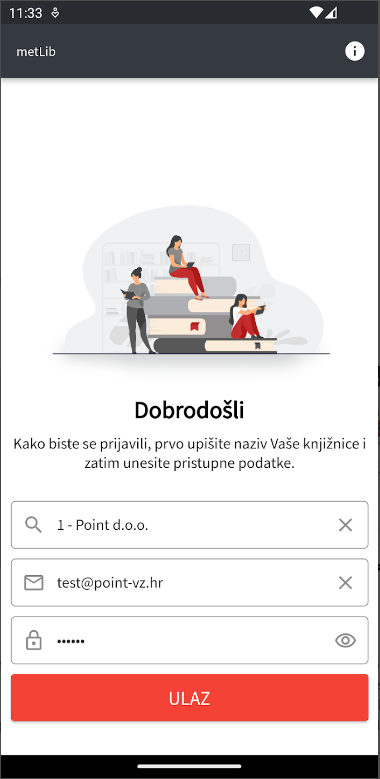
\includegraphics[scale=0.4]{slike/Login.PNG} %veličina slike u odnosu na originalnu datoteku i pozicija slike
		\centering
		\caption{Primjer prijave u aplikaciju}
		\label{fig:prijava}
	\end{figure}
	
	Web aplikacija ovog projekta imat će prozor za prijavu napravljenu po sličnom principu. Dok prikazana prijava uzima ime knjižnice, adresu e-pošte i lozinku kao što je prikazano na slici \ref{fig:prijava}, prijava projektne aplikacije uzimat će korisničko ime i lozinku te će se pomoću tih podataka prijavljivati prodavači knjiga.
		
	\subsection{Glavni prozor}
	
	Web aplikacija srodna projektnoj web aplikaciji ima više funkcionalnosti na glavnom prozoru nego što je predviđeno za projektnu web aplikaciju.

	\begin{figure}[H]
		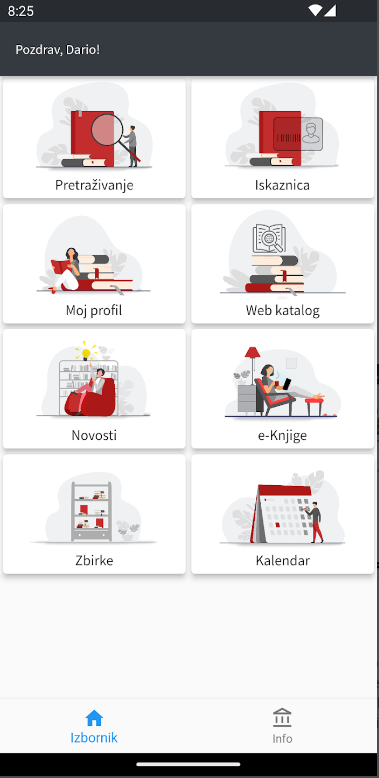
\includegraphics[scale=0.4]{slike/MainScreen.PNG} %veličina slike u odnosu na originalnu datoteku i pozicija slike
		\centering
		\caption{Primjer glavnog prozora}
		\label{fig:glavni prozor}
	\end{figure}	
	
	Dok prikazani prozor na slici \ref{fig:glavni prozor} uz pretraživanje knjiga ima gumbe koji vode na prozore za prikaz iskaznice, profil korisnika, web katalog, novosti, e-knjige, zbirke i kalendar, projektna web aplikacija primarno će imati prozor za prikaz liste knjiga i tražilicu pomoću koje će neregistrirani korisnici pretraživati bazu podataka unesenih knjiga. Dodatna funkcionalnost bit će mapa pomoću koje će korisnik birati različite prodavaonice ponuditelja nakon čega će mu se prikazati lista knjiga koje nudi ta prodavaonica. Registrirani korisnik umjesto ovog prozora imat će prozor s funkcionalnosti za unos i brisanje knjiga iz baze podataka.
	
	\subsection{Lista knjiga}
	
	Nakon što korisnik klikne na gumb za pretraživanje otvara se novi prozor s tražilicom i listom knjiga. Pretraga knjiga bit će omogućena po značajkama knjige i nazivu ponuditelja. Prozor na slici \ref{fig:lista knjiga} koji prikazuje listu knjiga u web aplikaciji metLib idealni je prikaz onoga što projektna web aplikacija nastoji proizvesti.
	
	\begin{figure}[H]
		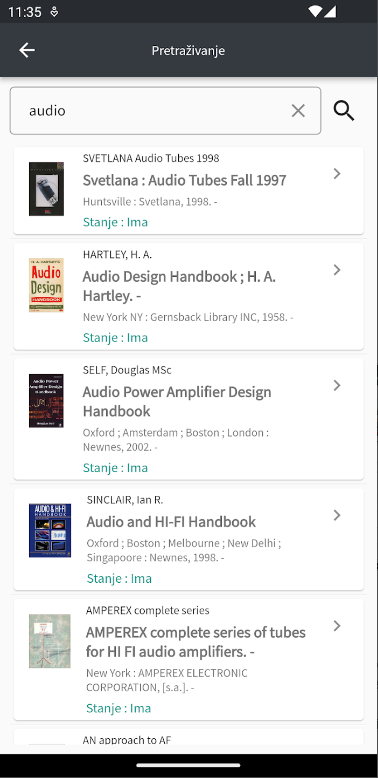
\includegraphics[scale=0.4]{slike/BookList.PNG} %veličina slike u odnosu na originalnu datoteku i pozicija slike
		\centering
		\caption{Primjer liste knjiga}
		\label{fig:lista knjiga}
	\end{figure}
	
	Neregistrirani korisnici na ovom će prozoru moći pretraživati knjige po značajkama i nazivu ponuditelja, dok će registrirani korisnici imati popis knjiga koje oni prodaju.
	
	\subsection{Prikaz knjige}
	
	Nakon odabira knjige u aplikaciji metLib otvara se ekran sa slike \ref{fig:prozor knjige} koji prikazuje koricu knjige, signaturu, autora, naslov, impresum, predmetnice i kratki opis. 
	
	\begin{figure}[H]
		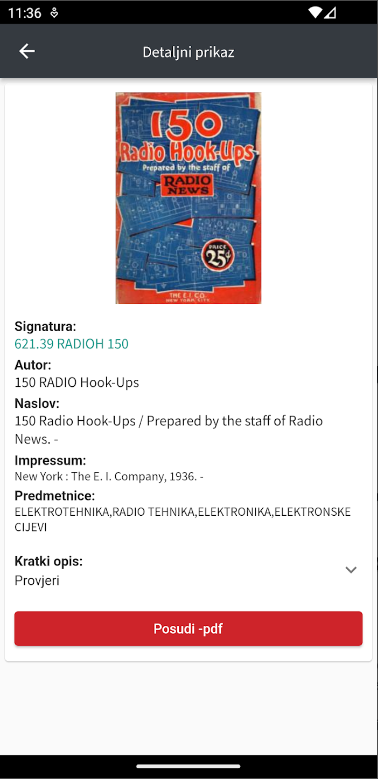
\includegraphics[scale=0.4]{slike/BookScreen.PNG} %veličina slike u odnosu na originalnu datoteku i pozicija slike
		\centering
		\caption{Primjer pregleda odabrane knjige}
		\label{fig:prozor knjige}
	\end{figure}
		
	Projektna web aplikacija također će sadržavati sličan feature gdje će neregistrirani korisnik odabirom knjige iz liste knjiga biti prebačen na prozor koji će sadržavati osnovne podatke o odabranoj knjizi: naziv, autore, godinu izdanja, izdavača, kategoriju izdavača, žanr, ISBN, broj izdanja, stanje očuvanosti, tekstni opis, sliku korica, oznaku vrste knjige i listu ponuda.
	
		
	